\documentclass[a4paper,openany]{memoir}

%%%%% Packages %%%%%
\usepackage{lmodern}
\usepackage{palatino}
\usepackage[T1]{fontenc}
\usepackage[utf8]{inputenc}

% To be removed if you want it in english
\usepackage[french]{babel}

\usepackage{amstext,amsmath,amssymb,amsfonts}
\usepackage{multirow,colortbl}
\usepackage{xspace,varioref}
\usepackage{hyperref, cite}

\usepackage[dvipsnames]{xcolor}
\usepackage{graphicx}

\usepackage{appendix}
\usepackage{makeidx}

%% custom style %%%%%%%%%%%%%%%%%%%%%%%%%%%%%%%%%%%%%%%%%%%%%%%%%%%%%%%%

% custom commands
\newcommand{\version}[1]{\def\theversion{#1}}
\newcommand{\subtitle}[1]{\def\thesubtitle{#1}}

\newcommand{\authors}[1]{\def\theauthors{#1}\author{#1}}
\newcommand{\supervisor}[1]{\def\thesupervisor{#1}}
\newcommand{\tutor}[1]{\def\thetutor{#1}}

% translation for custom words
\newcommand{\authorname}{Author}
\newcommand{\authorsname}{Authors}
\newcommand{\supervisorname}{Supervisor}
\newcommand{\tutorname}{Tutor}

\newcommand{\thepartname}{Part}

\ifdefined\addto{%
\addto{\captionsfrench}{\renewcommand{\authorname}{Auteur}}%
\addto{\captionsfrench}{\renewcommand{\authorsname}{Auteurs}}%
\addto{\captionsfrench}{\renewcommand{\supervisorname}{Superviseur}}%
\addto{\captionsfrench}{\renewcommand{\tutorname}{Tuteur}}}
\addto{\captionsfrench}{\renewcommand{\thepartname}{Partie}}
\else{}
\fi

%%%%% Setting Titlepage %%%%%
%%%%%%%%%%%%%%%%%%%%%%%%%%%%%
\pretitle{\flushleft\Huge\textsf}
\posttitle{\\[-.65em]\rule{\linewidth}{1.5mm}\\[-.65em]
\ifx\thesubtitle\undefined%
\else%
  \hfill{\small\itshape \thesubtitle}%
\fi
\centering
\vfill

\includegraphics{Universite_de_Bordeaux.pdf}
\vfill
\iflanguage{french}{
{\Huge Projet de deuxième année}
}{
 {\Huge Master2 Project}
}\\
\vspace{1.25em}
\iflanguage{french}{%
  \LARGE
  Master \emph{Sciences et Technologies},\\
  Mention \emph{Informatique},\\
% Mention \emph{Mathématiques},\\
  Parcours \emph{Cryptologie et Sécurité Informatique}.\\
  \par\hfill%
}{%
  \LARGE
  Master in \emph{Sciences and Technologies},\\
  Specialty in \emph{Computer Science},\\
% Specialty in \emph{Mathematics},\\
  Track \emph{Cryptology and Computer Security}.\\
  \par\hfill
}}

%% author
\preauthor{\vspace{\fill}\\
\ifx\theauthors\undefined%
  \flushleft\textbf{\large\authorname}\\
\else%
  \flushleft\textbf{\large\authorsname}\\
\fi
\small}
\postauthor{\vspace{1em}
\ifx\thesupervisor\undefined%
\else%
  \newline\textbf{\large\supervisorname}\\\thesupervisor\\[1em]%
\fi
\rule{\linewidth}{1mm}\\[-.25em]}

%% version and date
\predate{\hspace{\fill}
\ifx\theversion\undefined%
\else%
  version~\theversion~--~%
\fi}
\postdate{}

%% chapters style %%%%%%%%%%%%%%%%%%%%%%%%%%%%%%%%%%%%%%%%%%%%%%%%%%%%%%
%% You may try several styles (see more in the memoir manual).

%\chapterstyle{veelo}
%\chapterstyle{chappell}
%\chapterstyle{ell}
%\chapterstyle{ger}
%\chapterstyle{pedersen}
%\chapterstyle{verville}
\chapterstyle{madsen}
%\chapterstyle{thatcher}

%% parts style %%%%%%%%%%%%%%%%%%%%%%%%%%%%%%%%%%%%%%%%%%%%%%%%%%%%%%%%%

\renewcommand*{\thepart}{\arabic{part}}

\renewcommand*{\parttitlefont}{\chaptitlefont\HUGE}
\renewcommand*{\partnamefont}{\chapnamefont\huge}
\renewcommand*{\partnumfont}{\chapnumfont\huge}

\renewcommand{\beforepartskip}{\vspace*{\fill}}
\renewcommand{\midpartskip}{\vspace{.5em}\hrule height 0.5mm \vspace{.5em}}
\renewcommand{\afterpartskip}{\vspace*{\fill}}

% table of contents
\renewcommand*{\cftpartname}{\thepartname}
\renewcommand*{\cftpartpresnum}{\space}
\renewcommand*{\cftpartaftersnum}{.}
\renewcommand*{\cftpartaftersnumb}{\space}

\cftpagenumbersoff{part}
\renewcommand{\cftpartafterpnum}{\protect\\[-.75em]%
  \protect\mbox{}\protect\hrule\par}

\renewcommand{\cftchapterdotsep}{4}


%% index generation %%%%%%%%%%%%%%%%%%%%%%%%%%%%%%%%%%%%%%%%%%%%%%%%%%%%
\makeindex

%%%%% Useful macros %%%%%
\newcommand{\latinloc}[1]{\ifx\undefined\lncs\relax\emph{#1}\else\textrm{#1}\fi\xspace}
\newcommand{\etc}{\latinloc{etc}}
\newcommand{\eg}{\latinloc{e.g.}}
\newcommand{\ie}{\latinloc{i.e.}}
\newcommand{\st}{\ensuremath{\text{\xspace s.t.\xspace}}}


%%%%% Report Title %%%%%
\title{Attaque sur SSL/TLS}
\subtitle{Poodle et Triple-Handshake RSA}

\authors{Youri Laforgue \texttt{<youri.laforgue@etu.u-bordeaux.fr>}\\
Stewie Suivant \texttt{<stewie.suivant@etu.u-bordeaux.fr>}}

\supervisor{Abdou Guermouche \texttt{abdou.guermouche@labri.fr}}


%%%%%%%%%%%%%%%%%%%%%%%%%%%%%%%%%%%%%%%%%%%%%%%%%%%%%%%%%%%%%%%%%%%%%%%
%%%%%%%%%%%%%%%%%%%%%%%%%%%%%% Document %%%%%%%%%%%%%%%%%%%%%%%%%%%%%%%
%%%%%%%%%%%%%%%%%%%%%%%%%%%%%%%%%%%%%%%%%%%%%%%%%%%%%%%%%%%%%%%%%%%%%%%

\begin{document}

\frontmatter%%%%%%%%%%%%%%%%%%%%%%%%%%%%%%%%%%%%%%%%%%%%%%%%%%%%%%%%%%%
\maketitle
 \thispagestyle{empty}

 \cleardoublepage
\par\vspace*{\fill}

\iflanguage{french}{%
\section*{Déclaration de paternité du document}
}{%
\section*{Declaration of authorship of the document}}

\ifx\theauthors\undefined%
\iflanguage{french}{%
  Je certifie sur l'honneur que ce document que je soumet pour
  évaluation afin d'obtenir le diplôme de Master en \emph{Sciences et
    Technologies}, Mention \emph{Mathématiques} ou
  \emph{Informatique}, Parcours \emph{Cryptologie et Sécurité
    Informatique}, est entièrement issu de mon propre travail, que
  j'ai porté une attention raisonnable afin de m'assurer que son
  contenu est original, et qu'il n'enfreint pas, à ma connaissance,
  les lois relatives à la propriété intellectuelle, ni ne contient de
  matériel emprunté à d'autres, du moins pas sans qu'il ne soit
  clairement identifié et cité au sein de mon document.
  \bigskip

  \hfill\textbf{Date et Signature}
}{%
  I hereby certify that this material, which I now submit for
  assessment on the programme of study leading to the award of the
  Master in \emph{Sciences and Technologies}, Specialty in
  \emph{Mathematics} or \emph{Computer Science}, Track
  \emph{Cryptology and Computer Security}, is entirely my own work,
  that I have exercised reasonable care to ensure that the work is
  original, and does not to the best of my knowledge breach any law of
  copyright, and has not been taken from the work of others save and
  to the extent that such work has been cited and acknowledged within
  the text of my work.
  \bigskip

  \hfill\textbf{Date and Signature}}
\else%
\iflanguage{french}{%
  Nous certifions sur l'honneur que ce document que nous soumettons
  pour évaluation afin d'obtenir le diplôme de Master en
  \emph{Sciences et Technologies}, Mention \emph{Mathématiques} ou
  \emph{Informatique}, Parcours \emph{Cryptologie et Sécurité
    Informatique}, est entièrement issu de notre propre travail, que
  nous avons porté une attention raisonnable afin de nous assurer que
  son contenu est original, et qu'il n'enfreint pas, à notre
  connaissance, les lois relatives à la propriété intellectuelle, ni
  ne contient de matériel emprunté à d'autres, du moins pas sans qu'il
  ne soit clairement identifié et cité au sein de notre document.
  \bigskip

  \hfill\textbf{Date et Signatures}
}{%
  We hereby certify that this material, which we now submit for
  assessment on the programme of study leading to the award of the
  Master in \emph{Sciences and Technologies}, Specialty in
  \emph{Mathematics} or \emph{Computer Science}, Track
  \emph{Cryptology and Computer Security}, is entirely our own work,
  that we have exercised reasonable care to ensure that the work is
  original, and does not to the best of our knowledge breach any law
  of copyright, and has not been taken from the work of others save
  and to the extent that such work has been cited and acknowledged
  within the text of our work.\bigskip

  \hfill\textbf{Date and Signatures}}
\fi
\vspace{6em}


 \cleardoublepage
\tableofcontents*

\mainmatter%%%%%%%%%%%%%%%%%%%%%%%%%%%%%%%%%%%%%%%%%%%%%%%%%%%%%%%%%%%%


\chapter*{Introduction}

\paragraph{}
SSL (Secure Sockets Layer) et TLS (Transport Layer Security) définissent des protocoles 
permettant de sécuriser des échanges sur internet. SSL a été initiallement développé 
par Netscape en 1995, avec la version SSL 2.0. L'IETF prend le relais à la suite de la 
version SSL 3.0, et renomme le protocole TLS. La dernière version à ce jour est 
TLS 1.2 sorti en 2008.

Pour des raison de compatibilité, la majeure partie de ces versions sont 
encore utilisé à l'heure actuel.

\paragraph{}
TLS Fonctionne en mode client-serveur, et permet de répondre à plusieurs objectifs :
\begin{itemize}
\item L'authentification du serveur et/ou du client (authentification mutuelle).
\item La confidentialité des données échangées.
\item L'intégrité des données échangées.
\end{itemize}



\paragraph{}
Son objectif initial et principal est de sécuriser le protocole HTTP, 
notamment pour sécuriser les paiements en ligne lors de l'essort du e-commerce. 
Aujourd'hui, son champs d'application s'est étendu : protection d'autres 
protocoles comme SMTP ou LDAP, création de VPN, etc...

\paragraph{}
Ce protocole étant largement utilisé par les serveurs et navigateurs web 
pour la sécurisation des échanges sur internet, 
il est également la cible de nombreuse attaques visant à voler une connexion, 
usurper une identité, écouter le trafic pour récolter des informations sensibles 
(mot de passe, information bancaire, etc...).

\paragraph{}
Nous allons faire, dans un premier temps, 
le tour des attaques découvertes à partir de 2011, reposant sur différents mécanismes. 
Dans un deuxième temps, nous rentrerons dans le détails de deux attaques récentes, 
à savoir POODLE et 3-Handshake, verrons leur implémentation et aborderons 
les contres-mesures envisageables. 
Nous conclurons en ......................................................... .


\addcontentsline{toc}{chapter}{Introduction}


\part{Attaques sur SSL/TLS}

Cette partie est un état de l'art des attaques sur SSL depuis plusieurs années.
Elles peuvent être classifier en différentes catégorie :

\begin{itemize}
\item POA (Padding Oracle Attack)
\item Compression Attack
\item Timming Attack
\item Alogorithm Weakness Attack
\item Autres
\end{itemize}

Toutes ses attaques utilisent des faiblesses d'implémentations.
Ses attaques cherchent à obtenir la connaissance de données chiffrées
sans craquer l'algorithme de chiffrement. 

La plupart nécéssitent d'être en MITM (man in the middle) pour pouvoir
fonctionner. Il est parfois nécéssaire de pouvoir injecter du code 
sur le client.

Ses contraintes peuvent parraitre compliquées à mettre en place.
Dans les faits, Il est facile d'injecter du code sur un client
grâce à/à cause d'une utilisation de plus en plus courante du langage
javascript sur internet.


%%%%%%%%%%%%%%%%%%%%%%%%%%%%%%%%%%%%%%%%%%%
%%%%%%%%%%%%%%%%%%% POA %%%%%%%%%%%%%%%%%%%
%%%%%%%%%%%%%%%%%%%%%%%%%%%%%%%%%%%%%%%%%%%


\chapter{Padding Oracle Attack}
\label{chapter:poa}

\section{Présentation}
\label{sec:pPOA}

Cette attaque\up{\cite{article:poa}} a pour objectif de retrouver le clair d'un bloc chiffré 
avec le mode CBC\up{\ref{fig:cbc}}. Elle s'appuie sur le fait que le dernier bloc chiffré
contient du padding. De plus le dernier octet de padding corespond à la
taille du padding.\\
L'oracle  déchiffre le clair et vérifie que la taille du padding est correcte. 
Il renvoie une erreur en cas de taille erronée.\\

\section{Comment ça marche}
\label{sec:ccmPOA}

Supposons maintenant que l'attaquant possède un chiffré composé de 4 blocs :
$C_1||C_2||C_3||C_4$. Le bloc $C_4$ contient un padding de taille $x$ connu par l'attaquant.
il souhaite connaître le contenu de $C_2$ et quand il interroge l'oracle, celui-ci lui dit
si la taille est correcte ou non.\\
L'attaquant peut envoyer une version contrefaite du chiffré comme suit :
$C_1||C_2||C_3'||C_4'$.\\
\begin{itemize}
\item le bloc $C_4'=C_2$
\item le bloc $C_3'= C_3$ dont le dernier octet est modifié
\end{itemize}
Soit $P_n$ le déchiffrement de $C_n$ par l'oracle et D() et E() les algorithmes
de déchiffrement et de chiffrement. 
Le bloc qui nous intéresse est $P_4'$.
\[P_4' = D(C_2) + C_3'\]
or $C_2 = E(P_2 + C_1)$ d'où

\[\Longleftrightarrow P_4' = D(E(P_2 + C_1)) + C_3'\]
\[\Longleftrightarrow P_4' = P_2 + C_1 + C_3'\]
\begin{itemize}
\item $C_1$ et $C_3'$ sont connus
\item $P_2$ est le clair recherché
\item $P_4'$ est inconnu mais l'oracle nous dit si le dernier octet est égal à $x$.
\end{itemize}
Soit k la taille des blocs et Pn[i] le ième octet du bloc n.

\[P_4'[k] = P_2[k] + C_1[k] + C_3'[k]\] si $P_4'[k] = x$ alors
\[\Longleftrightarrow x = P_2[k] + C_1[k] + C_3'[k]\]
\[\Longleftrightarrow P_2[k] = x + C_1[k] + C_3'[k]\]

Ce qui donne une équation à une seule inconnue, donc l'attaquant a trouvé $P_2[k]$.
Pour avoir $P_4' = x$, il suffit de faire varier la valeur de $C_3'[k]$. Il est donc
possible de trouver le dernier octet de $P_2$ en un maximum de 256 essais.\\

Pour trouver les autres octets, l'attaquant prend $P_4'[k] = P_2[i]$ où $i \in [1,k]$.
Avec cette méthode il est possible de retrouver tout le contenu d'un chiffré à
l'exception du premier bloc (sauf si il est possible de modifier l'IV est connu).\\

\section{Contre-Mesures}
\label{sec:cmPOA}

Cette attaque n'est pas utilisable telle quelle sur SSL car elle demande de modifier un octet
d'un bloc qui n'est pas du padding. Cela entraîne un échec du déchiffrement du bloc, le
paquet sera donc rejeté à la vérification avec la MAC. Elle est toutefois le point de
départ de nombreuses attaques sur SSL/TLS dont Poodle\up{\ref{part:poodle}}
.


\chapter{BEAST}
\label{chapter:Beast}

\section{Présentation}
\label{sec:pBeast}

BEAST\up{\cite{article:study}} (Browser Exploit Against SSL/TLS) est une attaque  découverte par Rizzo et Duong en septembre 2011.
Elle se base sur une vulnérabilité de CBC trouvée en 2004 par Gregory V. Bard\up{\cite{article:bard}}. De plus, elle utilise une faille dans les
navigateurs qui permet de violer le SOP (Same Origin Policy).

Le SOP est un concept des applications web qui spécifie qu'une page web A ne peut accéder aux données d'une page web
B seulement si elles ont la même origine. S'il n'était pas appliqué, un site malveillant pourrait accéder aux
données d'un autre et voler des informations à un utilisateur.

Le mode CBC décrit plus bas\up{\ref{fig:cbc}}, est le mode de chiffrement par bloc utilisé par SSL/TLS. 
M. Bard a montré en 2004 que le protocole était vulnérable dans le cas d'une attaque CPA (choosen Plaintext Attack).

CBC utilise un IV (initialisation vector), celui-ci permet de chiffrer plusieurs fois le même message clair
et d'obtenir des chiffrés différents. Dans SSL/TLS, l'IV correspond au dernier au bloc de chiffré du message précédent.
Un attaquant qui observe le réseau est donc capable de connaitre l'IV qui sera utilisé pour le prochain message.

\section{Comment ça marche}
\label{sec:ccmBeast}

Dans le cas d'une attaque CPA, il est possible d'envoyer des messages à clairs choisis et d'obtenir leurs chiffrés
via un oracle de chiffrement. Dans notre contexte, cela revient à demander à la cible d'envoyer des messages, et
d'observer ce qui est envoyé sur le réseau.

Un attaquant qui connait l'IV et qui peut créer ses messages peut essayer de retrouver le clair d'un bloc avec une 
recherche exhaustive :

\begin{itemize}
\item Soit $C = C_1 || C_2 || C_3 || C_4$, un message intercepté par l'attaquant
\item Soit $P_i = D(C_i) + C_{i-1}$ avec $1 \leq i \leq 4$ 
\item Soit $C_i = E(P_i + C_{i-1}) $
\item L'attaquant cherche $P_3$
\end{itemize}

L'attaquant génère un message $P'$ comme suit :
\[ P' = C_4 + P_3' + C_2 || \dots\]
Ce qui donne le chiffré suivant :
\[ C' = E(P_3' + C_2 + C_4 + IV) || \dots  \]
or $C_4 = IV$
\[ C' = E(P_3' + C_2) || \dots \]
Si $P_3' = P_3 $ alors $C_1' = C_3$, l'attaquant peut donc par recherche exhaustive retrouver le bloc $P3$. Il peut
procéder ainsi pour tous les blocs. 

Il faudrait pour des blocs de taille 16 (AES-128) $256^{16} = 2^{128}$ messages pour déchiffrer un bloc. Il faut autant
d'essais que pour trouver la clé donc l'attaque n'est pas utile telle quelle.\\ 

Dans un message SSL/TLS, il est possible de connaître une partie du clair. Dans le cas de l'envoi d'un cookie de 
session, le message sera de la forme : \dots Cookie: sessid=dnu6YhPb5fd0kmQ \dots

Si l'attaquant veut voler le cookie de session, il peut utiliser l'attaque ci-dessus. la cible envoie une première
requête contenant le cookie de session tel qu'un des blocs soit "Cookie: sessid=d". Ce bloc posséde un seul octet
inconnu. Determiner cet octet avec l'attaque prendra au plus 256 essais.

Il suffit ensuite de faire envoyer à la cible le même message mais décalé comme suit : "ookie: sessid=dn", et
réitérer jusqu'à reconstituer tout le cookie de session. Pour un cookie de session de taille n, il faudra maximum
n * 256 essais.

\section{Contre-Mesures}
\label{sec:cmBeast}

   L'attaque repose sur deux pré-requis : la connaissance de l'IV et la CPA. 

Il est possible de retirer la connaissance de l'IV, il suffit de rajouter de l'aléatoire dans sa géneration. 
Si l'IV n'est plus prédictible, l'attaque ne fonctionne plus. Cela est le cas à partir de TLS 1.1 et plus.

Si L'attaquant ne peut pas outrepasser le SOP, il ne peut plus faire de CPA. Les navigateurs ont fixé ce problème mais
il existe toujours des moyens de l'outrepasser ( cross-origin request, ...). 





\chapter{Lucky 13}
\label{chapter:luck}

En cryptanalyse, une timing attack\up{\cite{article:Timming}} est une attaque par cannaux cachés dans laquelle 
un attaquant tente de compromettre un crypto-système en analysant le temps d'exécution 
de l'algorithme cryptographique. TIME, BREACH  et Lucky13 en font partie.

\section{Présentation}
\label{sec:pL13}

Cette attaque\up{\cite{article:study}} a été mise en évidence par Nadhem AlFardan and Kenny Paterson, le 4 Février 2013.

Elle est basée sur le padding Oracle Attack\up{\ref{chapter:poa}}. Le problème de POA est qu'il n'est pas possible de déterminer
quand le padding est correct. En effet, quand celui-ci est validé, le serveur vérifie le MAC qui a été modifié par l'attaquant.

Dans lucky 13, l'idée est de se servir du temps de réponse pour obtenir cette information. C'est une TIMMING-ATTACK.
Elle requiert d'être en MITM et pouvoir injecter du code sur le client.

\section{Comment ça marche}
\label{sec:ccmL13}

Soit un message M de 77 octets reçu par le serveur, \[ M = Sequence (8) || Header (5) || Data (D = 44 -p) || MAC (20) || PADDING (p) \]

Quand le serveur reçoit un message M, il le déchiffre et vérifie la taille du padding. 
Ensuite il doit hasher  $M = Sequence (8) || Header (5) || Data (D = 44 - p)$  et le comparer au MAC 
pour vérifier l'intégrité. Afin de savoir où se termine les données, il se sert de la taille du Padding.

Il y a trois cas possible : 
\begin{itemize}
\item Le padding a une taille invalide alors p vaut 0 octet. $D=44$
\item le padding a une taille valide de 0. $D=43$ 
\item la padding a une taile valide de 1.$D=42$
\end{itemize}

Le seveur va hashé son message pour le vérifier au MAC. Les hashs utilisés par SSL
ont des blocs de 64 octets, donc si un message fait plus de 64 octets, il aura deux
opération de hashs. De plus, c'est fonction ajoute au message au moins 1 octet de 
padding et 8 octets pour la longueur.

Dans notre cas, le hash fait 13 + D + 9. Ce qui donne respectivement pour nos trois cas :
66, 65 et 64 octet. Le troisième aura une seule opération de MAC et deux pour les autres.
Il est possible avec une TIMMING Attack de voir la différence. 

L'attaque Lucky 13 se base sur ça pour son attaque. Quand elle repére une différence
notable, elle peut appliquer la formule du Padding Oracle Attack.

\section{Contre-Mesures}
\label{sec:cmL13}

Une contre-mesure simple serait de rajouter des délais dans les temps de réponses,
ou bien de les uniformiser.

De toute façon, cette attaque n'est pas réalisable car la différence est difficilement observable. 
 % TIMMING

%%%%%%%%%%%%%%%%%%%%%%%%%%%%%%%%%%%%%%%%%%
%%%%%%%%%%%%%% Compression %%%%%%%%%%%%%%%
%%%%%%%%%%%%%%%%%%%%%%%%%%%%%%%%%%%%%%%%%%

\chapter{CRIME}
\label{chapter:crime}

\paragraph{}
CRIME (Compression Ratio Info-leak Made Easy) est une attaque visant TLS, découverte en .... par les memes chercheurs que BEAST (Juliana Rizzo et Thai Duong). Cette attaque vise à récupérer de l'information lors d'une connexion sécurisée par TLS. Typiquement, l'attaquant cherche à découvrir le cookie de session de la victime afin d'usurper par la suite son identité.

\paragraph{}
Pour que l'attaque aboutisse, 2 conditions sont nécessaires :
\begin{itemize}
  \item L'attaquant doit etre placé en MITM (Man In The Middle).
  \item L'attaquant doit pouvoir injecter du code (javascript) dans le navigateur de la victime.
\end{itemize}

\paragraph{}
TLS propose, dans sa version ?.?, la compression. C'est à dire que les données à transmettre sont tout d'abord compressées, puis chiffrées avant d'etres transmisent sur internet.

L'idée, c'est que l'attaquant va envoyer une requête via le navigateur de la victime, en y intégrant des données à lui.

Pour illustrer ce qui se passe, prenons 2 chaines de caractères :
\begin{itemize}
\item C1 => ATTACKERDATA:x UNKNOWNCOOKIE:y OTHERDATA»
\item C2 => ATTACKERDATA:y UNKNOWNCOOKIE:y OTHERDATA»
\end{itemize}
On apperçoit une redondance de la lettre 'y' dans C2, ce qui implique qu'après compression, C2 sera plus courte que C1. Le chiffrement ne modifiant pas la taille de la chaine, le chiffré de C2 sera également plus court que le chiffré de C1. Il y'a donc une fuite d'information.

\paragraph{}
Le code javascript injecter va envoyer des requêtes vers le serveur maBanque.fr, en y ajoutant 'Cookie: sessionid=a'. Le navigateur de la victime va alors intégrer le vrai cookie dans la requete (voir ci-dessous).


\begin{verbatim}
POST /anyurl HTTP/1.1
Host: bank.com
(…)
Cookie: sessionid=d8e8fca2dc0f896fd7cb4cb0031ba249
(…)
sessionid=a
\end{verbatim}


La requête est alors compressée puis chiffrée. L'attaquant regarde la taille du chiffré.
Lorsque qu'il tente d'ajouter 'sessionid=d', le chiffré sera plus court (voir ci-dessous). 


\begin{verbatim}
POST /anyurl HTTP/1.1
Host: bank.com
(…)
Cookie: sessionid=d8e8fca2dc0f896fd7cb4cb0031ba249
(…)
sessionid=d
\end{verbatim}

Il suffit de répéter l'opération pour trouver les caractères suivants. L'attaquant peut ainsi reconstituer le cookie d'authentification.

\paragraph{}
Pour corriger cette faille, il suffit simplement de désactiver l'option de copression sur le serveur et le client.


\chapter{TIME}
\label{chapter:time}


\section{Présentation}
\paragraph{}
TIME\up{\cite{article:study}} est une attaque à clair choisi découverte par Tal Be'ery et Amichai Shulman. A l'instar de CRIME qui utilise comme fuites d'information la taille des chiffrées, TIME utilise le temps.

Suite aux corrections apportées à TLS après la découverte de CRIME, les attaques ne peuvent plus se baser sur la compression TLS. Cependant, la compression au niveau du protocole HTTP est toujours active, et ce pour des soucis d'optimisation de bande passante. C'est donc le temps de compression des données au niveau du serveur que l'attaquant va mesurer.

\section{Comment ça marche}
\paragraph{}
Les seuls pré-requis nécessaires pour l'attaquant sont :
\begin{itemize}
  \item D'injecter un script pour forger les requêtes du client.
  \item D'avoir un moyen de mesurer précisemment les temps de réponse du serveur.
\end{itemize}

L'attaquant n'a plus besoin de se mettre en MITM. Le calcul du temps de réponse est directement fait au niveau du script injecté.

\paragraph{}
Un facteur essentiel à prendre en compte pour une attaque réussie est le RTT (Round-Trip Time). Cette information représente le temps entre le moment où le client envoie une requête et le moment où il reçoit l'acusé de reception. Si un paquet IP est supérieur à 1500 octets, ce qui correspond au MTU (Maximum Transmission Unit) sur internet, celui-ci  sera fragmenté et aura potentiellement un RTT supérieur à un paquet non fragmenté (inférieur à 1500 octets). Cette différence de RTT entre ces 2 paquets est assez significative pour être décelée. Une dernière information à prendre en compte est le fenêtrage TCP. Pour un gain de performance, il est possible d'envoyer T paquets sans avoir reçu un seul ACK. Le T+1 paquet est alors bloqué et doit attendre la reception du 1er ack pour que la fenêtre d'envoie coulisse.\\

Pour qu'un attaquant puisse mettre en place cette attaque, il va forcer la longueur des données compressées jusqu'au seuil de fragmentation du paquet. Ainsi, selon que l'octet à deviner soit bon ou pas, la compression sera plus ou moins performante, et le paquet sera ou non fragmenté. De plus, il faut qu'il comble toute la fenêtre TCP. Ainsi, tout paquet additionnel due à une mauvaise valeur de l'octet recherché rajoutera un RTT avec un delai relativement significatif.
Pour un octet valide, le RTT sera alors plus court que pour un octet invalide.

\paragraph{}
Il est fort probable que du bruit soit présent sur le réseau. Si c'est le cas, pour chaque valeur d'un octet à deviner, il sera utile d'envoyer plusieurs fois la même requête et de considérer le temps de réponse minimale comme la valeur du RTT. Le RTT le plus court pour les différentes valeur d'un octet est alors considérée comme la bonne valeur.\\

De proche en proche, l'attaquant peut récupérer le cookie de session de la victime et toutes autres données secrètes insérées dans le corps de la réponse.

\section{Contre-Mesures}
\paragraph{}
Pour que cette attaque fonctionne, il faut que l'ajout de l'attaquant dans le header soit également présent dans le corps de la réponse. Si c'est le cas, la compression sera efficace, sinon, rien ne sera mesurable par l'attaquant.

\paragraph{}
Cette attaque étant une fois de plus due à des problèmes d'implémentations, les contre-mesures suivante sont ciblées sur cette dernière :
\begin{itemize}
  \item Ajouter un delai aléatoire lors du déchiffrement peut rendre plus compliquer la recherche de la donnée secrète.
  \item Désactiver la compression au niveau de HTTP. Cependant, ce n'est pas faisable sans impacter la performance et la rapidité des serveurs web.
  \item Les contrôles doivent êtres plus rigoureux dans l'utilisation des entrées utilisateur dans les réponses HTTP.
  \item Utiliser des techniques pour limiter les requêtes répétitives.
\end{itemize}
 % TIMMING

\chapter{BREACH}
\label{chap:breach}

\paragraph{}
BREACH à été présenté en aout 2013 par Yoel Gluck, Neal Harris et Angelo Prado. Là où CRIME vérifie la taille des données compressées par TLS, là où TIME va mesurer le temps de réponse des données compressées par HTTP, BREACH va regarder la taille des réponses compressées par HTTP. Contrairement à CRIME, cette attaque ne vise pas le cookie de session. Cela est due au fait le cookie de session se trouve dans l'entête HTTP alors que la compression HTTP ne cible que le corps de la réponse et non l'entête. Les informations secrètes pouvant êtres extraites doivent donc êtres présentes dans le corps de la réponse.\\

L'algorithme de compression utilisé est DEFLATE. Il utilise lui-même 2 autres algorithme : LZ77 et le codage de Huffman.

\paragraph{}
Les prérequis pour satisfaire cette attaque sont celles de CRIME :
\begin{itemize}
  \item Pouvoir forger les requêtes du client.
  \item Se retrouver en MITM.
\end{itemize}

\paragraph{}
L'attaquant va envoyer une requête contenant dans l'entête 'CSRFtoken=x'. ce Bout de code sera alors présent dans le corps de la réponse, ainsi que la vrai valeur du CSRF. Lorsque le serveur web va compresser le corps de la réponse, si la valeur x est bonne, le chiffré sera plus court que si elle ne l'est pas. L'attaquant teste donc toute les valeurs de 'x' possible jusqu'à tomber sur un chiffré plus court que les autres. De proche en proche, il peut retrouver la valeur entière de la donnée secrète recherchée.\\

Pour exemple, voilà ci-dessous une requète servant à trouver la valeur du CSRFtoken :

\begin{verbatim}
GET /product/?id=1234&user=CSRFtoken=x HTTP/1.1
Host: exemple.fr
(…)
\end{verbatim}

Et voilà la réponse HTTP du serveur web :

\begin{verbatim}
<form target="https://exemple.fr:443/products/catalogue.aspx?id=1234&user=CSRFtoken=x HTTP/1.1">
(...)
<td nowrap id="tdErrLgf">
<a href="logoff.aspx?CSRFtoken=4bd634cda846fd7cb4cb0031ba249ca2">Log Off</a>
</td>
(…)
\end{verbatim}

L'attaquant remarquera que la taille minimale des chiffrés des réponses HTTP est effective pour x = '4', et pourra considérer cette valeur comme exacte pour le 1er octet du jeton CSRF. De proche en proche, il peut retrouver la valeur entière de la donnée secrète recherchée.


 % TIMMING

%%%%%%%%%%%%%%%%%%%%%%%%%%%%%%%%%%%%%%%%%%
%%%%%%%%%%%%%%%%%%% BUG %%%%%%%%%%%%%%%%%%
%%%%%%%%%%%%%%%%%%%%%%%%%%%%%%%%%%%%%%%%%%

\chapter{Triple-Handshake RSA}
\label{chapter:RSA}

\section{Présentation}
\label{sec:pTHR}

l'attaque\up{\cite{article:handshake}} a été découverte par Antoine Delignat-Lavaud, Karthikeyan Bhargavan et Alfredo Pironti 
de l'équipe de recherche Prosecco de INRIA Paris-Rocquencourt. 

Elle est présenté comme une nouvelle classe d'attaque. Un client se connecte sur un serveur malicieux et le serveur
se connecte sur un serveur cible en se faisant passer pour le client. C'est une attaque MITM sur trois Handshake.
L'attaquant réussit l'attaque s'il réussit à se faire passer pour le client après la troisième poignée de main.


\section{Comment ça marche}
\label{sec:ccmTHR}

L'attaque se passe en trois étapes :

\subsection{Etape 1}
\label{sec:e1}

\begin{figure}[h]
\label{fig:hand1}
\centering
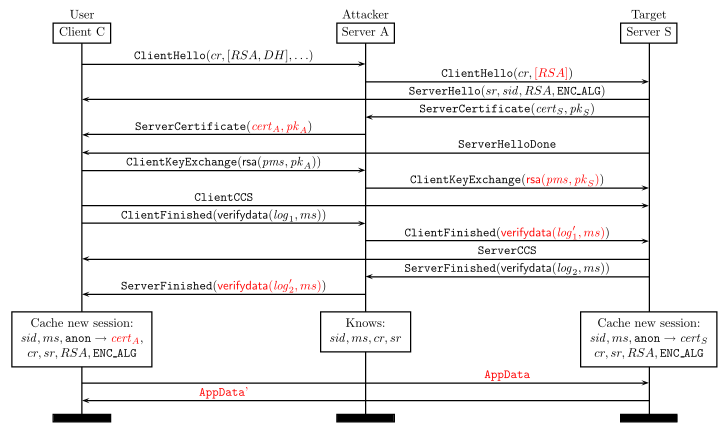
\includegraphics[scale=0.4]{Hand1}
\caption{Triple Handshake : Etape 1}
\end{figure}

Le client $C$ se connecte sur le serveur malicieux $A$. Dans le même temps, $A$ se connecte au serveur $S$ en utilisant
les informations de connexion de $C$. L'attaquant change la requête ClientHello pour imposer le choix de RSA. $A$
doit donner à $C$ et $S$ ses certificats.

$A$ va alors pouvoir récupérer le PMS ( Pre Master Secret ), et le réemettre au serveur. Il doit ensuite modifier
les logs. Ces messages sont les premiers à être chiffré et contiennent un hashé de l'ensemble 
des messages échangés pendant la négociation. Il doit donc les modifiés pour les faire corespondre au log de $C$ et $S$.

L'attaquant a deux connexions avec les mêmes paramètres et clés mais avec des certificats serveur et des logs 
différents. La première poignée de main est finie.

\subsection{Etape 2}
\label{sec:e2}

\begin{figure}[h]
\label{fig:hand2}
\centering
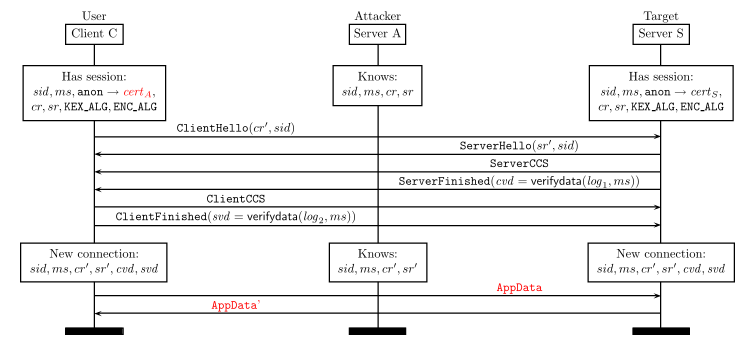
\includegraphics[scale=0.5]{Hand2}
\caption{Triple Handshake : Etape 2}
\end{figure}

$C$ se reconnecte à $A$ et demande un résumé de la connexion précédente. $A$ se reconnecte en retour à $S$ et demande la même chose.
Ensuite $A$ va seulement retransmettre les messages de $C$ vers $S$ et inversement.

A la fin de cette deuxième poignée de main, $C$ et $S$ ont maintenant les mêmes logs. Ils ont aussi négocier de
nouvelles clés, mais comme $A$ est au milieu, il les connait. 
\pagebreak

\subsection{Etape 3}
\label{sec:e3}

\begin{figure}[h]
\label{fig:hand3}
\centering
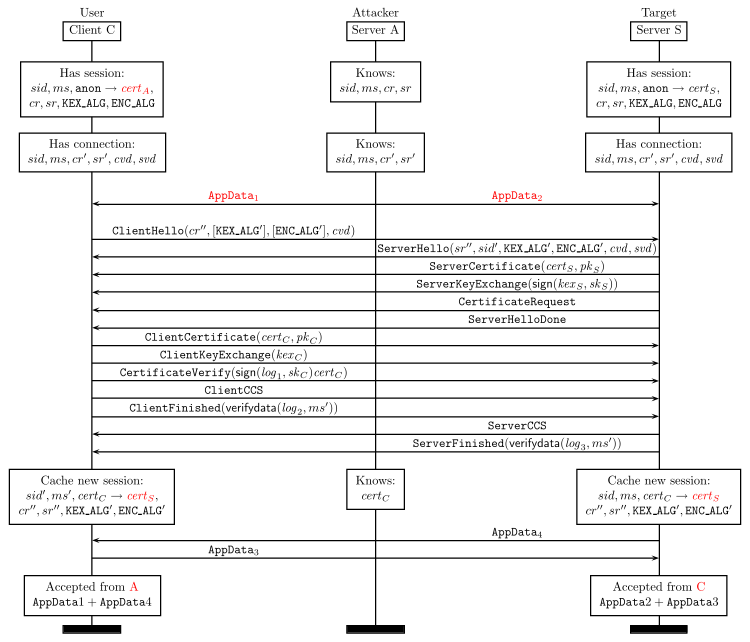
\includegraphics[scale=0.4]{Hand3}
\caption{Triple Handshake : Etape 3 }
\end{figure}

$S$ demande la renégociation complète avec authentification à $A$, qui envoi la demande à $C$. $A$ va seulement faire suivre les messages. A la
fin de la rénégociation, les données de connexion de $C$ et $S$ sont les mêmes. $S$ va envoyer son certificat à $C$.
En principe, $C$ devrait rejetter ce certificat mais en réalité il est accepté par de nombreux navigateurs. La raison
est simple, un serveur peut changer de certificat, parce qu'il a expiré par exemple.

Toutefois, $A$ n'a plus connaissance de la clé de session ou de la nouvelle master key. En effet, pour evoyer
le master secret, $C$ a utilisé la clé publique du certificat de $S$ donc $A$ ne peut pas la déchiffrer.
 Il ne peut donc pas agir ou observer les communications entre le client et le serveur. 

Cette vulnérabilité n'est pas exploitable seule. Cependant, $A$ peut par exemple retransmettre l'image exacte du site de $S$ en
y intégrant un script qui permet d'utiliser une attaque outrepassant le SOP.


\section{Contre-Mesures}
\label{sec:cmTHR}

Pour éviter ces attaques, il faudrait revoir la politique de TLS vis à vis du changement des certificats.
Il faudrait interdire de changer les certificats durant une renégociation. Ainsi la troisième étape ne 
fonctionnerait plus.

Une autre possibilité est de rajouter au master secret un hash du précédent handshake. Ainsi lors d'une
renégociation, le client et le serveur peuvent vérifier leur intégrité respective. Dans notre attaque, 
le hash sera éronné puisque $C$ aura l'identité de $A$ au lieu de $S$, de même pour $S$.

 



\chapter{FREAK}
\label{chap:freak}

\section{Présentation}
\label{sec:pFreak}

L'attaque FREAK\up{\cite{article:freak1}} (Factoring RSA-Export Key, le A peut être pour Apple ou Android), découverte
par Karthikeyan Bhargavan et l'équipe miTLS\up{\cite{article:freak2}} de l'inria de Paris, le 3 mars 2015.


Cette vulnérabilité résulte d'une exigence de la NSA dans les années 90. Elle imposait des chiffrements
facilement décryptables par eux aux produits vendus à l'étranger.
Ces algorithmes furent baptisés "RSA-Export" et utilisaient des clés RSA de 512 bits.


Bien entendu, ces algorithmes ne sont plus utilisés dans les implémentations actuelles, mais pour un souci de retro-compatibilité, ils subsistent toujours dans OpenSSL.

\section{Comment ça marche}
\label{sec:ccmFreak}

Dans SSL/TLS, lors de la négociation de clé, l'algorithme de chiffrement choisi et censé être le plus
robuste commun aux deux communiquants. Si l'attaquant est en MITM, il est capable de modifier la requête ClientHello.
Cette requête envoie au serveur sa liste d'algorithmes disponibles. Cette liste est remplacée par RSA-Export. Le serveur
va alors créer une clé de taille 512 bits et celle-ci sera acceptée par le client.

L'attaquant est en MITM, il peut donc observer le réseau et récupérer les clés publiques. Il lui reste alors à 
chercher la factorisation de n. Il lui sera ensuite possible de déchiffrer tous les messages chiffrés entre le
client et le serveur

Trouver la factorisation d'une clé de 512 bits peut sembler difficile mais si l'attaquant est en mesure d'utiliser
des gros serveurs de calcul, il peut le faire rapidement. A titre d'exemple, l'équipe miTLS, estime à 12 heures le temps de calcul avec un serveur Amazon EC2. Cette clé sera valide uniquement le temps de la session donc 12 heure 
peut paraître long mais dans les faits les clés de session ne changent pas souvent.

\section{Contre-Mesures}
\label{sec:cmFreak}

Cette attaque a besoin que le serveur et le client accepte d'utiliser les clés RSA-Export.

Les serveurs qui acceptent ces clés représentent environ 26 \% des serveurs SSL/TLS\up{\cite{article:freak3}}. Une mise à jour a été faite par
TLS pour bloquer ces clés.

Au niveau des navigateurs, tous ne sont pas vulnérables. Les principaux sont Safari, chrome Android et IE. 
A l'heure actuelle, chrome Android est toujours vulnérable, IE est patché et safari l'est en partie.

\chapter{Heartbleed}
\label{chapter:Heartbleed}

\paragraph{}
Heartbleed, présente depuis mars 2012, à été révélée en avril 2014 par l'équipe de sécurité de Google et des ingénieurs de Codenomicon (société finlandaise). C'est une vulnérabilité logicielle due à une erreur de programmation dans la librairie openSSL. Contrairement aux attaques précédentes qui cible assez clairement les informations à extraire, Heartbleed ne permet pas de choisir ce que l'on veut récupérer. Un attaquant utilisant cette attaque peut lire la mémoire d'un serveur ou d'un client et peut récupérer aussi bien des clés privées que des choses sans importances.




%%%%%%%%%%%%%%%%%%%%%%%%%%%%%%%%%%%%%%%%%%%%%%%%%%%%%%%%%%%%%%%%%%%%%%%

\part{Poodle}
\label{part:poodle}

\chapter{Présentation}
\label{chapter:poodlePres}

L'attaque Poodle (Padding Oracle On Downgraded Legacy Encryption)

a été découverte par Bodo Möller, Thai Duong et 
Krzysztof Kotowicz\cite{article:ssl-poodle} en septembre 2014.\\

Cette attaque se base sur une faiblesse de SSLv3.
Elle fonctionne pourtant sur les dernières versions de TLS.
Pour maintenir la compatibilité avec tout les clients, un
serveur TLS peut rétrograder en version SSLv3.\\

C'est une attaque de typer Man-In-The-Middle (l'homme du milieu).
L'attaquant peut utiliser un site malveillant qui injecte un
code javascript sur le client pour le faire générer des requêtes
sur le serveur cible. Il peut alors forcer l'utilisation de 
SSLv3, même si le client et le serveur utilisent TLS.\\

L'objectif de l'attaque est de voler le cookie de session 
du client. Pour cela, comme BEAST, l'attaquant force 
l'utilisation du mode CBC. Elle utilise le \emph{padding oracle attack }

\chapter{Padding Oracle Attack}
\label{chapter:POA}

Cette attaque a pour objectif de retrouver le clair d'un bloc chiffré 
avec le mode CBC. Elle s'appuie sur le fait que le dernier bloc chiffré
contient du padding. De plus le dernier octet de padding corespond à la
taille du padding.\\

L'oracle  déchiffre le clair et vérifie que la taille du padding est correcte. 
Il renvoie une erreur en cas de taille erronée.\\

Supposons maintenant que l'attaquant posséde un chiffré composé de 4 blocs :
$C1||C2||C3||C4$. Le bloc $C4$ contient un padding de taille $x$ connu par l'attaquant.
il souhaite connaitre le contenu de $C2$ et quand il interoge l'oracle, celui-ci lui dit
si la taille est correcte ou non.\\
L'attaquant peut envoyer une version contrefaites du chiffré comme suit :
$C1||C2||C3'||C4'$.\\
\begin{itemize}
\item le bloc $C4'=C2$
\item le bloc $C3'= C3$ dont le dernier octet est modifié
\end{itemize}
Soit $Pn$ le déchiffrement de $Cn$ par l'oracle et D() et E() les algorithmes
de déchiffement et de chiffrement. 
Le bloc qui nous intérésse est $P4'$.
\[P4' = D(C2) + C3'\]
or $C2 = E(P2 + C1)$ d'où
\[\Longleftrightarrow P4' = D(E(P2 + C1)) + C3'\]
\[\Longleftrightarrow P4' = P2 + C1 + C3'\]
\begin{itemize}
\item $C1$ et $C3'$ sont connus
\item $P2$ est le clair recherché
\item $P4'$ est inconnu mais l'oracle nous dit si le dernier octet égale à $x$.
\end{itemize}
Soit k la taille des blocs et Pn[i] le iéme octet du bloc n.

\[P4'[k] = P2[k] + C1[k] + C3'[k]\] si $P4'[k] = x$ alors
\[\Longleftrightarrow x = P2[k] + C1[k] + C3'[k]\]
\[\Longleftrightarrow P2[k] = x + C1[k] + C3'[k]\]

Ce qui donne une equation a une seule inconnu donc l'attaquant a trouvé $P2[k]$.
Pour avoir $P4' = x$, il suffit de faire varier la valeur de $C3'[k]$. Il est donc
possible de trouver le dernier octet de $P2$ en maximum de 256 essais.\\

Pour trouver les autres octets, l'attaquant prend $P4'[k] = P2[i]$ où $i \in [1,k]$.
Avec cette méthode il est possible de retrouver tout le contenu d'un chiffré à
l'exeption du premier bloc (sauf si l'IV est connu).

\chapter{Mise en place de l'attaque}
\label{chapter:Poodleattack}





%%%%%%%%%%%%%%%%%%%%%%%%%%%%%%%%%%%%%%%%%%%%%%%%%%%%%%%%%%%%%%%%%%%%%%%


\chapter*{Conclusion}
\label{chapter:ccl}

SSL s'est plein de failles donc c'est \textbf{NUL}.



%%%%%%%%%%%%%%%%%%%%%%%%%%%%%%%%%%%%%%%%%%%%%%%%%%%%%%%%%%%%%%%%%%%%%%%%


\part*{Annexes}
\addcontentsline{toc}{part}{Annexes}
\appendix

\backmatter%%%%%%%%%%%%%%%%%%%%%%%%%%%%%%%%%%%%%%%%%%%%%%%%%%%%%%%%%%%%

\nocite{*}
\bibliographystyle{plain}
\bibliography{bibliography}

\printindex

\end{document}
